\section{NPN Circuit with E resistance}
In Figure \ref{lab3_ex9_de}, calculate all the values of $I_B$, $I_C$, $I_E$, $V_E$, and $V_C$. Assume the voltage drop $V_{BE}$ = 0.7V and the current gain coefficient of the transistor is $\beta$ = 100. Then, perform a simulation to double-check your theoretical calculations.

\begin{figure}[h]
    \centering
    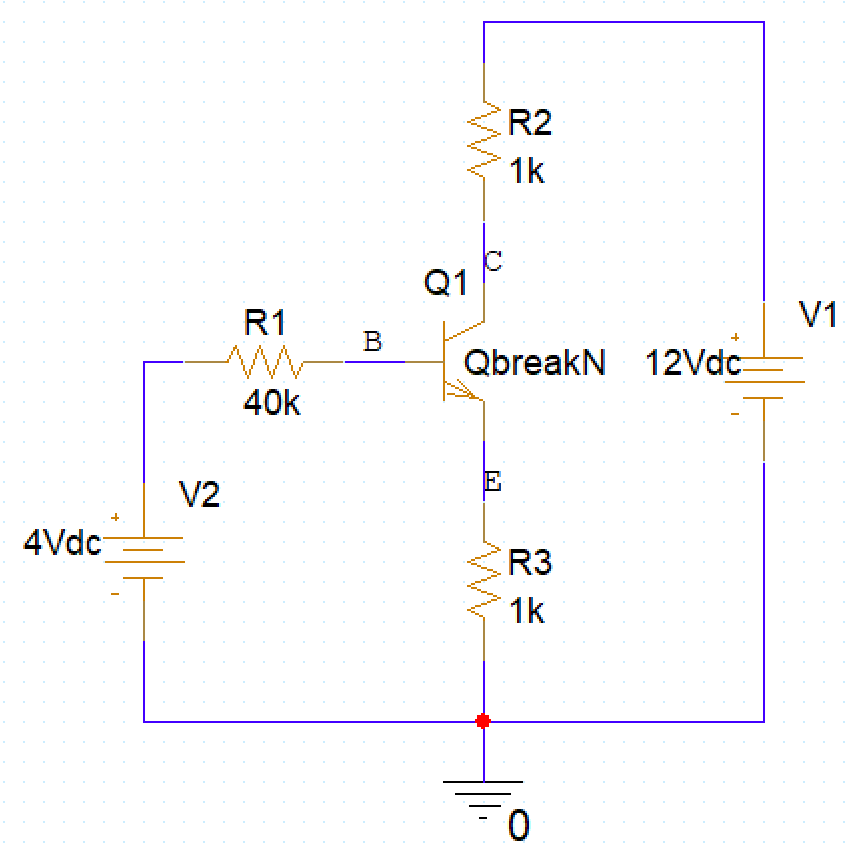
\includegraphics[width=10cm]{graphics/ex8/lab3_ex9_de.png}
    \caption{NPN Circuit with E resistance}
    \label{lab3_ex9_de}
\end{figure}

\subsection{Theoretical calculation}
Note:

Explanations, formulas, and equations are expected rather than only results.

Theo KVL, KCL, định luật Ohm, ta có các phương trình sau:
\[
40000 \cdot I_B + V_{BE} + 1000 \cdot I_E = V_2
\]
\[
\Leftrightarrow 40000 \cdot I_B + V_{BE} + 1000(\beta + 1) \cdot I_B = V_2 \quad (1)
\]
Giải (1), ta có: 
\[
I_B = \frac{V_2 - V_{BE}}{41000 + 1000 \cdot \beta} = 23.4 \, \mu \text{A}
\]
\[
I_C = \beta \cdot I_B = 2.34 \, \text{mA}
\]
\[
I_E = (\beta + 1) \cdot I_B = 2.36 \, \text{mA}
\]
\[
V_E = I_E \cdot R_3 = 2.36 \, \text{V}
\]
\[
V_C = V_1 - I_C \cdot R_2 = 9.66 \, \text{V}
\]

\subsection{Simulation}
Your image goes here
\begin{figure}[h]
    \centering
    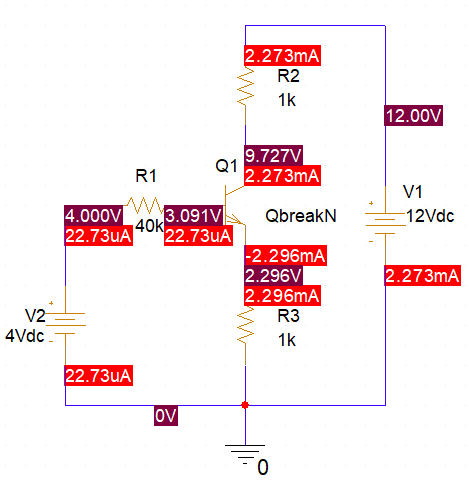
\includegraphics[width=0.5\textwidth]{graphics/ex8/f1.PNG}
\end{figure}